\documentclass[notes,11pt, aspectratio=169]{beamer}

\usepackage{pgfpages}
% These slides also contain speaker notes. You can print just the slides,
% just the notes, or both, depending on the setting below. Comment out the want
% you want.
\setbeameroption{hide notes} % Only slide
%\setbeameroption{show only notes} % Only notes
%\setbeameroption{show notes on second screen=right} % Both

%\usepackage[scaled=1.0]{helvet}
\usepackage{array}


\usepackage{tikz}
\usetikzlibrary{calc}
\usetikzlibrary{matrix}
\usetikzlibrary{positioning}

\newcommand{\payoff}[4][below]{\node[#1]at(#2){$(#3,#4)$};}
\usepackage{verbatim}
\setbeamertemplate{note page}{\pagecolor{gray!5}\insertnote}
\usetikzlibrary{positioning}
\usetikzlibrary{snakes}
\usetikzlibrary{calc}
\usetikzlibrary{arrows}
\usetikzlibrary{decorations.markings}
\usetikzlibrary{shapes.misc}
\usetikzlibrary{matrix,shapes,arrows,fit,tikzmark}
\usepackage{amsmath}
\usepackage{mathpazo}
\usepackage{hyperref}
\usepackage{lipsum}
\usepackage{multimedia}
\usepackage{graphicx}
\usepackage{multirow}
\usepackage{graphicx}
\usepackage{dcolumn}
\usepackage{bbm}
\newcolumntype{d}[0]{D{.}{.}{5}}

\usepackage{changepage}
\usepackage{appendixnumberbeamer}
\newcommand{\beginbackup}{
   \newcounter{framenumbervorappendix}
   \setcounter{framenumbervorappendix}{\value{framenumber}}
   \setbeamertemplate{footline}
   {
     \leavevmode%
     \hline
     box{%
       \begin{beamercolorbox}[wd=\paperwidth,ht=2.25ex,dp=1ex,right]{footlinecolor}%
%         \insertframenumber  \hspace*{2ex} 
       \end{beamercolorbox}}%
     \vskip0pt%
   }
 }
\newcommand{\backupend}{
   \addtocounter{framenumbervorappendix}{-\value{framenumber}}
   \addtocounter{framenumber}{\value{framenumbervorappendix}} 
}


\usepackage{graphicx}
\usepackage[space]{grffile}
\usepackage{booktabs}

% These are my colors -- there are many like them, but these ones are mine.
\definecolor{blue}{RGB}{0,114,178}
\definecolor{red}{RGB}{213,94,0}
\definecolor{yellow}{RGB}{240,228,66}
\definecolor{green}{RGB}{0,158,115}

\hypersetup{
  colorlinks=false,
  linkbordercolor = {white},
  linkcolor = {blue}
}

\usepackage{graphicx,stackengine,xcolor}
\newcommand\Circle[1]{%
	\def\useanchorwidth{T}%
	\def\stacktype{L}%
	\stackon[0pt]{#1}{\scalebox{2.0}[1.15]{\textcolor{red}{$\bigcirc$}}}%
}

%% I use a beige off white for my background
\definecolor{MyBackground}{RGB}{255,253,218}

%% Uncomment this if you want to change the background color to something else
%\setbeamercolor{background canvas}{bg=MyBackground}

%% Change the bg color to adjust your transition slide background color!
\newenvironment{transitionframe}{
  \setbeamercolor{background canvas}{bg=white}
  \begin{frame}}{
    \end{frame}
}

\setbeamercolor{frametitle}{fg=blue}
\setbeamercolor{title}{fg=black}
\setbeamertemplate{footline}[frame number]
\setbeamertemplate{navigation symbols}{} 
\setbeamertemplate{itemize items}{-}
\setbeamercolor{itemize item}{fg=blue}
\setbeamercolor{itemize subitem}{fg=blue}
\setbeamercolor{enumerate item}{fg=blue}
\setbeamercolor{enumerate subitem}{fg=blue}
\setbeamercolor{button}{bg=MyBackground,fg=blue,}

%%% TIKZ STUFF
\tikzset{   
	every picture/.style={remember picture,baseline},
	every node/.style={anchor=base,align=center,outer sep=1.5pt},
	every path/.style={thick},
}
\newcommand\marktopleft[1]{%
	\tikz[overlay,remember picture] 
	\node (marker-#1-a) at (-.3em,.3em) {};%
}
\newcommand\markbottomright[2]{%
	\tikz[overlay,remember picture] 
	\node (marker-#1-b) at (0em,0em) {};%
}
\tikzstyle{every picture}+=[remember picture] 
\tikzstyle{mybox} =[draw=black, very thick, rectangle, inner sep=10pt, inner ysep=20pt]
\tikzstyle{fancytitle} =[draw=black,fill=red, text=white]
%%%% END TIKZ STUFF


% If you like road maps, rather than having clutter at the top, have a roadmap show up at the end of each section 
% (and after your introduction)
% Uncomment this is if you want the roadmap!
% \AtBeginSection[]
% {
%    \begin{frame}
%        \frametitle{Roadmap of Talk}
%        \tableofcontents[currentsection]
%    \end{frame}
% }
\setbeamercolor{section in toc}{fg=blue}
\setbeamercolor{subsection in toc}{fg=red}
\setbeamersize{text margin left=1em,text margin right=1em} 

\newenvironment{wideitemize}{\itemize\addtolength{\itemsep}{10pt}}{\enditemize}
\newenvironment{wideenumerate}{\enumerate\addtolength{\itemsep}{10pt}}{\endenumerate}

\usepackage{environ}
\NewEnviron{videoframe}[1]{
  \begin{frame}
    \vspace{-8pt}
    \begin{columns}[onlytextwidth, T] % align columns
      \begin{column}{.58\textwidth}
        \begin{minipage}[t][\textheight][t]
          {\dimexpr\textwidth}
          \vspace{8pt}
          \hspace{4pt} {\Large \sc \textcolor{blue}{#1}}
          \vspace{8pt}
          
          \BODY
        \end{minipage}
      \end{column}%
      \hfill%
      \begin{column}{.42\textwidth}
        \colorbox{green!20}{\begin{minipage}[t][1.2\textheight][t]
            {\dimexpr\textwidth}
            Face goes here
          \end{minipage}}
      \end{column}%
    \end{columns}
  \end{frame}
}

\title[]{\textcolor{blue}{ECN 453: Extra Game Theory Questions}}
\author[PGP]{}
\institute[FRBNY]{\small{\begin{tabular}{c c c}
Nicholas Vreugdenhil \\
\end{tabular}}}
\date{} 

\begin{document}

% Title Slide
\begin{frame}
\maketitle
  \centering
\end{frame}

\begin{frame}{The discrete Bertrand game (p186)}
	\begin{wideitemize}
		\item \textbf{Question}: Two firms set prices simultaneously. Consumers buy from the firm with the lowest price and split their demand equally across the two firms if prices are equal. Market demand is $q=10-p$, $MC=2$. Sellers can only set the following prices: $3,4,5$.
		\item 1. Write down the normal form game.
		\item 2. Solve for the equilibrium of the game.
	\end{wideitemize}
\end{frame}

\begin{frame}{Ex. 7.7 HDTV Standards}
	\begin{wideitemize}
		\item \textbf{Question:} US and Japan simultaneously decide whether to invest a high or low value into HDTV research. If both countries choose `low' payoffs are (4,3) for the US and Japan respectively. If US chooses low level and Japan a high level, payoffs are (2,4). If US chooses high level and Japan low, payoffs are (3,2). If both countries chooses a high level, payoffs are (1,1). 
		\item 1. Are there any dominant strategies in this game? What is the Nash equilibrium? What are the implicit rationality assumptions?
		\item 2. Suppose the US now has the option of committing to a strategy ahead of Japan. How would you model this situation? What are the subgame-perfect Nash equilbria of this game?
		\item 3. Comparing your answers to 1. and 2., what can you say about the value of commitment for the US?
	\end{wideitemize}
\end{frame}

\begin{frame}{Price match guarantee in the market for luxury cars}
	\begin{wideitemize}
		\item Two firms are competing on prices. Each firm can choose to set a high price $p_H$ or a low price $p_L$, where $p_H > p_L$. Profits are given by:
		\begin{figure}
			\centering
		 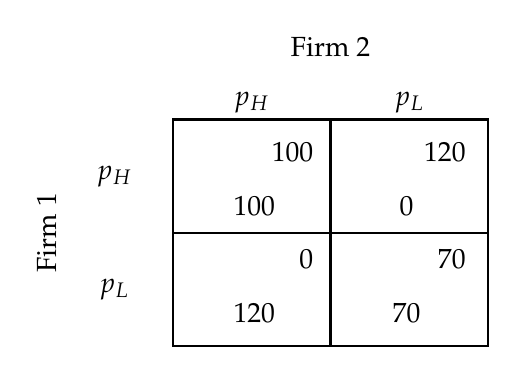
\begin{tikzpicture}
			\matrix[matrix of math nodes,every odd row/.style={align=right},every evenrow/.style={align=left},every node/.style={text width=1.5cm},row sep=0.2cm,column sep=0.2cm,ampersand replacement=\&] (m) {
				100 \& 120 \\
				100 \& 0 \\
				0 \& 70 \\
				120 \& 70 \\
			};
			\draw (m.north east) rectangle (m.south west); 
			\draw (m.north) -- (m.south);
			\draw (m.east) -- (m.west);
			
			% Player 1
			\coordinate (c) at ($(m.north west)!0.25!(m.south west)$);
			\coordinate (d) at ($(m.north west)!0.75!(m.south west)$);
			\node[left=2pt of c,text width=1cm]  {$p_H$};
			\node[left=2pt of d,text width=1cm]  {$p_L$};
			
			% Player 2
			\coordinate (a) at ($(m.north west)!0.25!(m.north east)$);
			\coordinate (b) at ($(m.north west)!0.75!(m.north east)$);
			\node[above=5pt of a,anchor=base] {$p_H$};
			\node[above=5pt of b,anchor=base] {$p_L$};
			
			\node[above=18pt of m.north] (firm b) {Firm 2};
			\node[left=1.6cm of m.west,rotate=90,align=center,anchor=center] {Firm 1};
			
			%\node[above=5pt of firm b]  {Payoff Matrix};
		\end{tikzpicture}
		\end{figure}
		\begin{wideitemize}
		\item 1. Draw the extensive form if firm 1 moves first. Solve for the subgame perfect equilibrium.
		\item 2. Suppose firm 1 offers consumers to match its price with the lowest price in the market. Solve for the SPE of the modified game (Hint: modify the game to three stages, allowing firm 1 to make a move in the third stage only in the case where it chose $p_H$ in the first stage and firm 2 chose $p_L$ in the second stage.)
		\end{wideitemize}
	\end{wideitemize}
\end{frame}


\end{document}
